%\documentclass[11pt,xcolor=gray,handout]{beamer}
\documentclass[hyperref={pdfpagelabels=false}]{beamer}
\let\Tiny=\tiny
\mode<presentation>{
\usetheme{Singapore}
%\usecolortheme{lily}
\usefonttheme{serif}
}
\usepackage{default}
\usepackage{verbatim}
%\usepackage{ucs}
\usepackage[utf8]{inputenc}
\usepackage{gb4e}
\usepackage[T1]{fontenc}
\usepackage{ tipa }
\usepackage{qtree}
\usepackage{synttree}
\usepackage{color}
\usepackage{tree-dvips}
\usepackage[absolute,overlay]{textpos}
%\usepackage{covington-beamer}
\usepackage{lmodern}
\usepackage{natbib}
\usepackage{graphicx}
%\usepackage{pdfpages}


%\usepackage{memoir}
%\usepackage{relsize}
%\newcommand{\subscript}[1]{\raisebox{-0.25em}{\smaller #1}}
%\logo{\includegraphics[height=0.5cm]{hilogo2.png}}
\setbeamertemplate{footline}[frame number] 
%gets rid of navigation symbols
\setbeamertemplate{navigation symbols}{}

\title{Allophonic Emergence: three ways allophonic rules come to be}
\author{Betsy Sneller and Joel C. Wallenberg \\ University of Pennsylvania, Newcastle University}
\institute{}
%\date[]{May 28, 2015 \\ something something Iceland}

\begin{document}

\begin{frame}[plain]
\titlepage
\end{frame}

\section{Introduction}
\begin{frame}{Introduction}
	An introductory thing about allophonic emergence. We will argue that there are 3 different types, and provide some things about things.
			
\end{frame}

\begin{frame}
\frametitle{Outline}
\tableofcontents
\end{frame}

\section{Three paths to allophony}
\subsection{Mechanical Means}

\begin{frame}{Mechanical Means}
	Traditionally assumed scenario \cite{ohala1983, ohala1989} \\
	\begin{itemize}
		\item A \textbf{mechanical}, subgrammatical effect skews the distribution of outputs perceived by the learner 
		\begin{itemize}
			\item Articulatory
			\item Perceptual
		\end{itemize}
	\end{itemize}
\end{frame}

%\subsubsection{Example: preaspiration in NW England English}}
\begin{frame}{Mechanical Means: \\ \small{Preaspiration in NW England English}}
Explanation of preaspiration in NW England English %\citep{Hejna2014}.

\end{frame}

\subsection{Spontaneous Phonologization}

\begin{frame}{Spontaneous Phonologization}
	Scenario proposed by (Joseph and Janda, Fruehwald) 
	
	\begin{itemize}
		\item Speakers \textbf{spontaneously} create an allophone without any phonetic motivation.  \\
		\begin{itemize}
			\item Allophonic categories emerge in individual speakers' grammars before any phonetic motivation
		\end{itemize}
	\end{itemize}
\end{frame}

%\subsubsection{Example: PRICE-raising in Philadelphia English}
\begin{frame}{Spontaneous Phonologization: \\ \small{PRICE-raising in Philadelphia English (Fruehwald 2013)}}

	Example about /ay/ raising in Philadelphia English
\end{frame}

\subsection{Phonological Specialization}

\begin{frame}{Phonological Specialization}

	Proposed by us!
	\begin{itemize}
		\item A phonetic change begins, creating variation in phonetic space
		\item This variation is reanalyzed as an allophonic distinction for a generation of speakers
		\begin{itemize}
				\item how it's different from Ohala, RBO
				\item How it's different from JJ, Frueh
		\end{itemize}
	\end{itemize}

\end{frame}

\subsubsection{Example: GOOSE-fronting in New Zealand English}
\begin{frame}{Phonological Specialization: \\ \small{GOOSE-NEW split in New Zealand English (Seyfarth and Sneller 2014)}}

\begin{center}
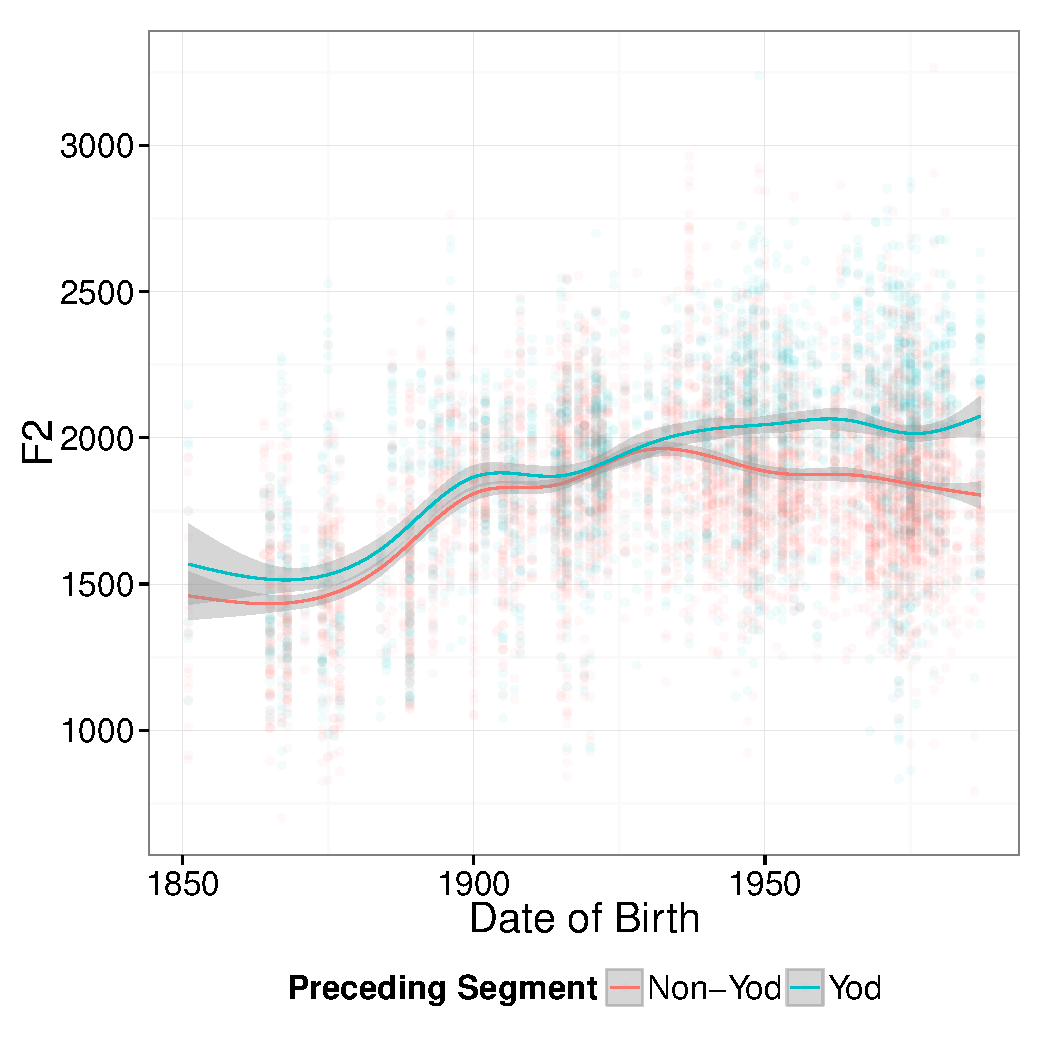
\includegraphics[width=.7\textwidth]{ByTokenOldPreceding.pdf}
\end{center}
\end{frame}

\section{Testing for the types}

\subsection{Effect of duration}
\begin{frame}{Effect of duration}
	Explanation about how we expect an effect of duration for phonetic differences
\end{frame}

\begin{frame}{Effect of duration}
	\begin{block}{Mechanical means}
		\begin{itemize}
			\item Because the allophonic split is the result of accruing phonetic effects, we should see a gradual decrease in the effect of duration over generational time 
			\item Other things
			\item hope this is in a block
		\end{itemize}
	\end{block}	
\end{frame}

\begin{frame}{Conclusions}
	\begin{block}{Conclusions}
		\begin{itemize}
			\item Within syntax, only one formal account of optionality is available, the same one that accounts for language change: Competing Grammars.
			\item This results in replacement, specialization, or stable variation (true optionality).
			\item The latter is (only) the result of mapping categorical variation onto a continuous dimension of specialization.
			\item An acquisition simulation shows how stable variation can emerge under a minimal Principle of Contrast.
			\item It is possible and desirable to extend this formal account to other domains of variation, like morphology and phonology.
		\end{itemize}
	\end{block}


\end{frame}

%\subsection{Rate of change}
%\begin{frame}{Rate of change}
%blahblah
%\end{frame}

%\begin{frame}[allowframebreaks]
%\frametitle{References}
%\newcommand*{\newblock}{natbib}
%\bibliographystyle{linquiry2}
%\bibliography{../tyneside/articles/joelrefs}
%\end{frame}
\end{document}